Испытания представляют собой процесс установления соответствия программы и
программной документации заданным требованиям.

\subsection{Проверка требований к документации}
Проверяется наличие всех документов перечисленных в пyнкте 4.1 данного
документа и их соответствие ГОСТ.

\subsection{Проверка требований к интерфейсу}
Интерфейс должен соответствовать схеме, указанной в настоящем Техническом
Задании и быть совместим а ОС Андроид. Использованные графические элементы
должны быть стандартными элементами графического семейства системы Андроид.
Используемая цветовая палитра должна соответствовать рекомендациям сайта,
указанного в настоящем Техническом Задании. Рис.~\ref{interface}

\begin{figure}[h!]
    \centering
    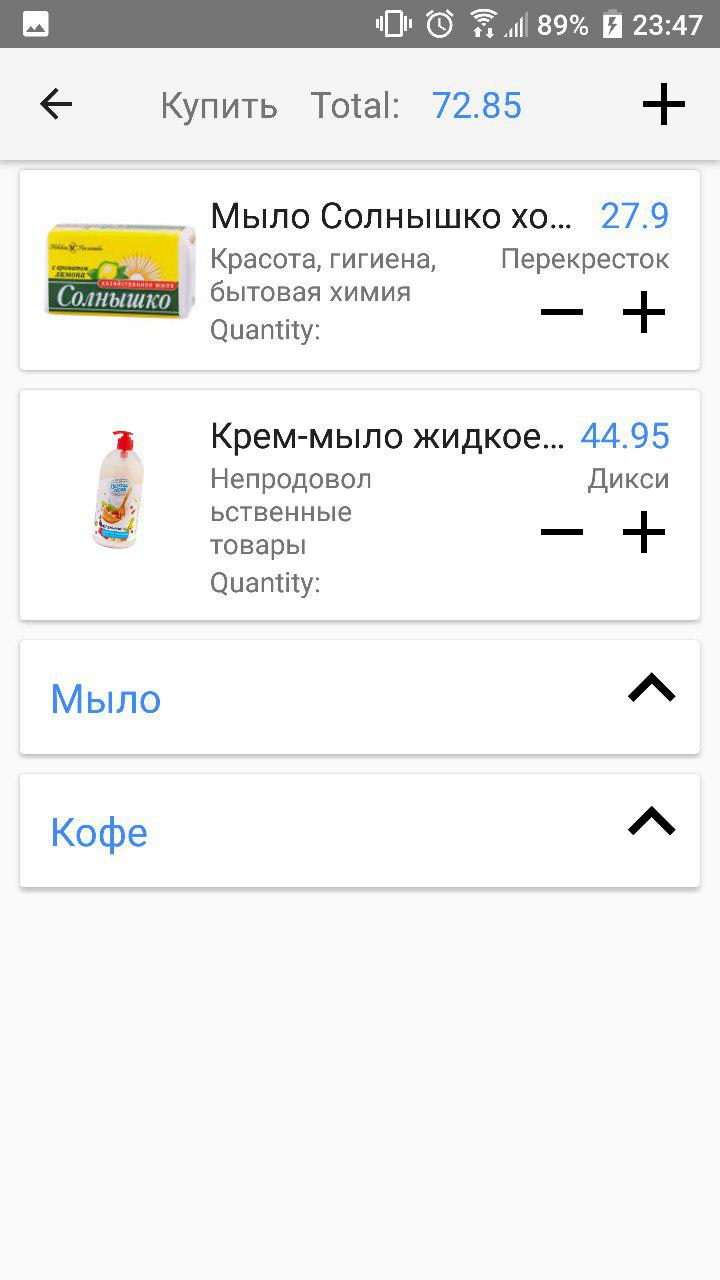
\includegraphics[height=0.48\textheight]{./screenshots/3/shoplist.jpg}
    \caption{проверка требований к интерфейсу}
    \label{interface}
\end{figure}

\newpage
\subsection{Проверка требований к функциональным характеристикам}

\subsubsection{Андроид приложение}
Проверка реализованного функционала продемонстрирована на скриншотах ниже.

Должна быть реализованa возможность просмотра списка доступных магазинов с
акционными товарами (выпадающий список на Рис.~\ref{items}), представление текущих акций для конкретного магазина в
виде общего списка и по категориям. (Рис.~\ref{categs_1},~\ref{categs_2}) Должна быть реализована постепенная
загрузкa товаров магазинов (по страницам) для экономии трафика и меньшей
нагрузкой на мобильное устройство.

Загрузка акций не должна превышать лимит, установленный требованиями и проверена в
пункте 6.4 настоящей Программы и Методики Испытаний.

\begin{figure}[h!]
    \centering
    \minipage{0.3\textwidth}
    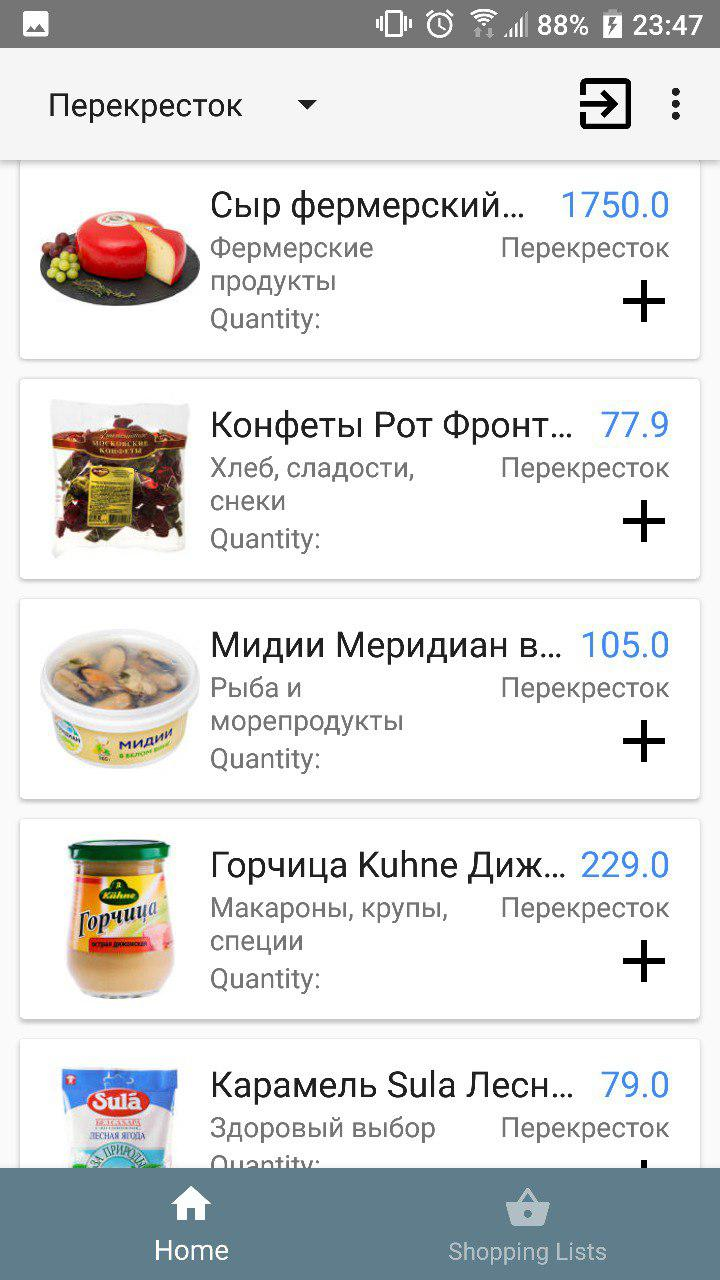
\includegraphics[height=0.38\textheight]{./screenshots/3/home.jpg}
    \caption{\small{просмотр всех акций}}
    \label{items}
    \endminipage\hfill
    \minipage{0.3\textwidth}
    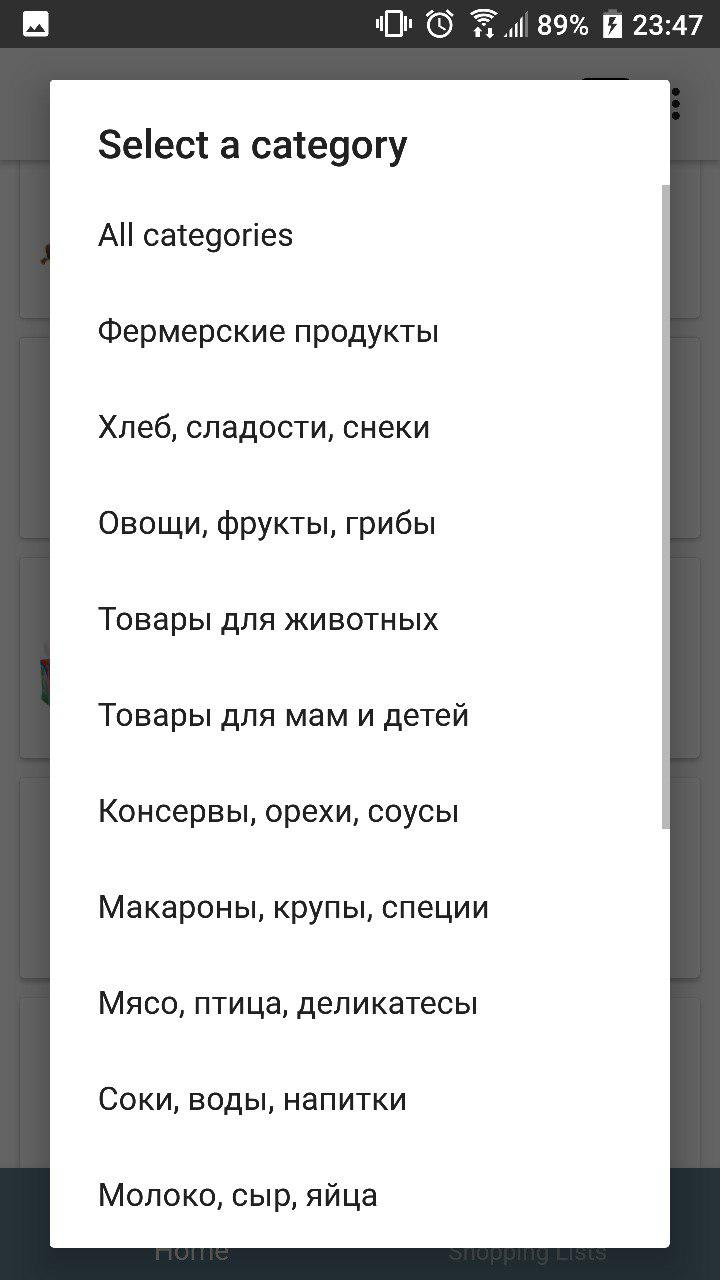
\includegraphics[height=0.38\textheight]{./screenshots/3/categories.jpg}
    \caption{\small{выбор категории}}
    \label{categs_1}
    \endminipage\hfill
    \minipage{0.3\textwidth}
    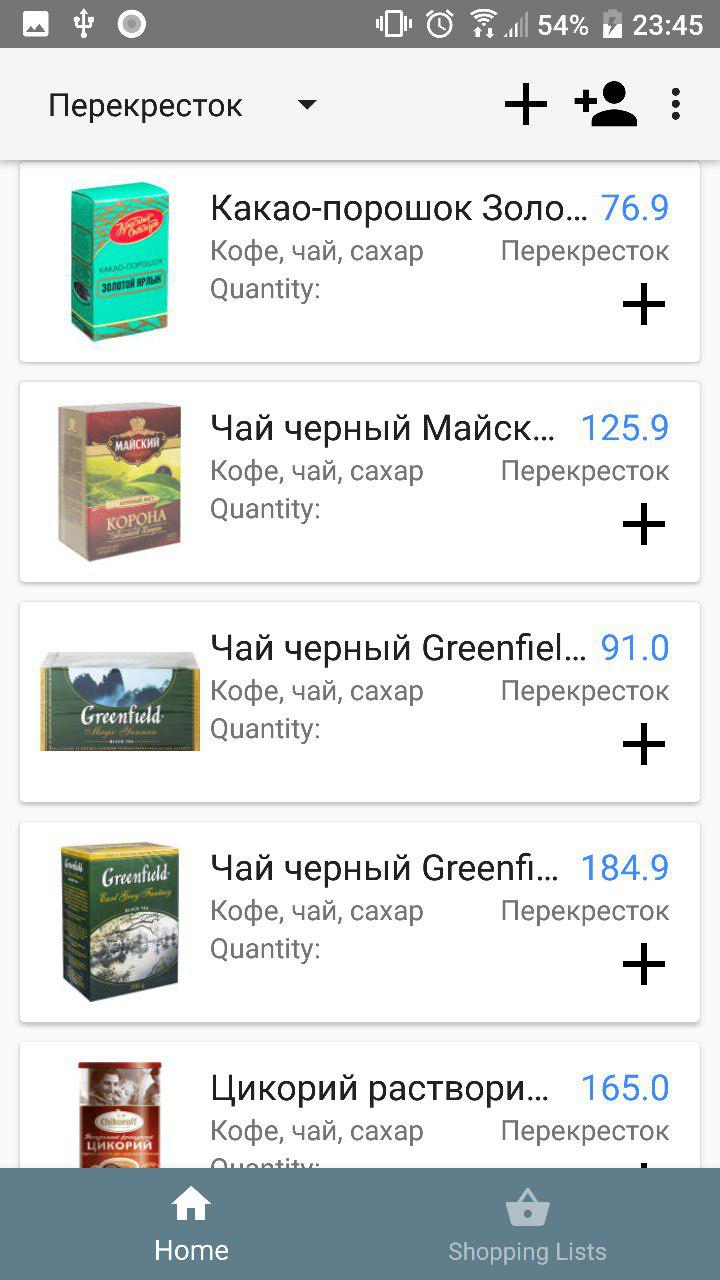
\includegraphics[height=0.38\textheight]{./screenshots/3/categ_filter.jpg}
    \caption{\small{просмотр по категориям. На скриншоте --- категория ``Кофе, чай, сахар''}}
    \label{categs_2}
    \endminipage{}
\end{figure}

Должна быть реализована возможность создания списков покупок c разными названиями,
и возможность удаления списка покупок. (Рис.~\ref{sl_all} -~\ref{delete_sl})

\begin{figure}[h!]
    \centering
    \minipage{0.3\textwidth}
    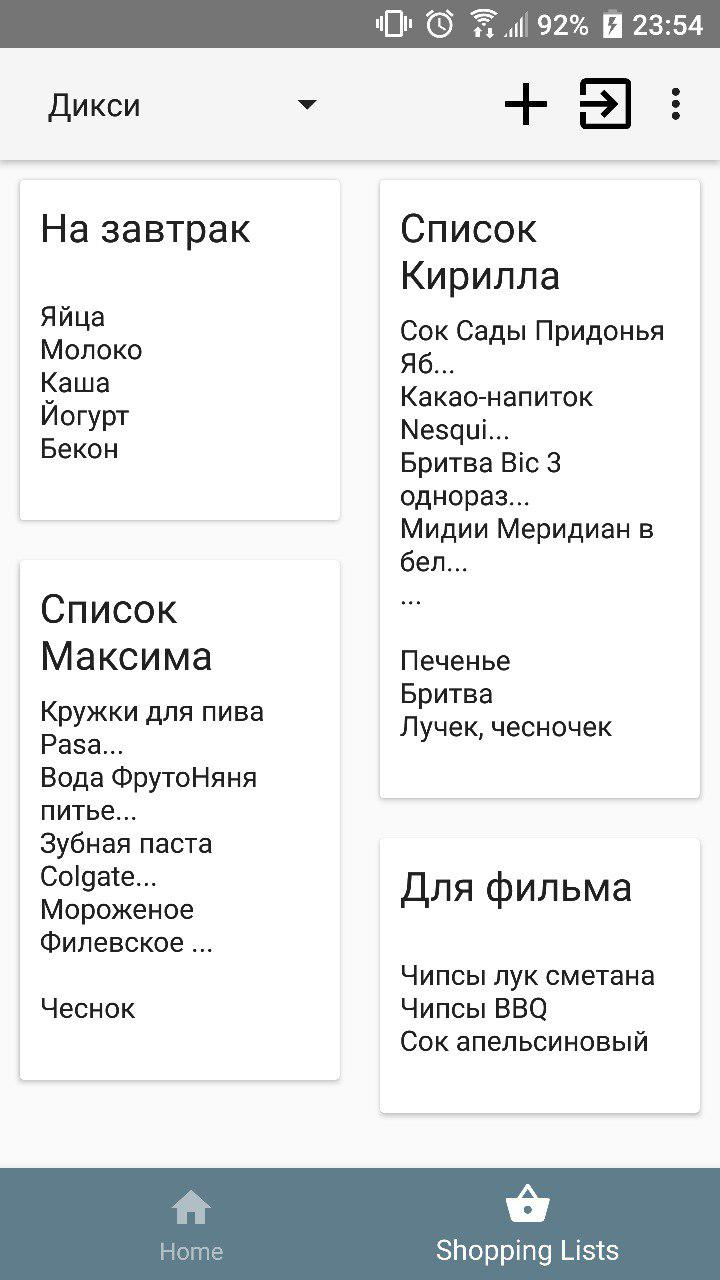
\includegraphics[height=0.38\textheight]{./screenshots/3/all_shoplists.jpg}
    \caption{\small{просмотр всех списков покупок}}
    \label{sl_all}
    \endminipage\hfill
    \minipage{0.3\textwidth}
    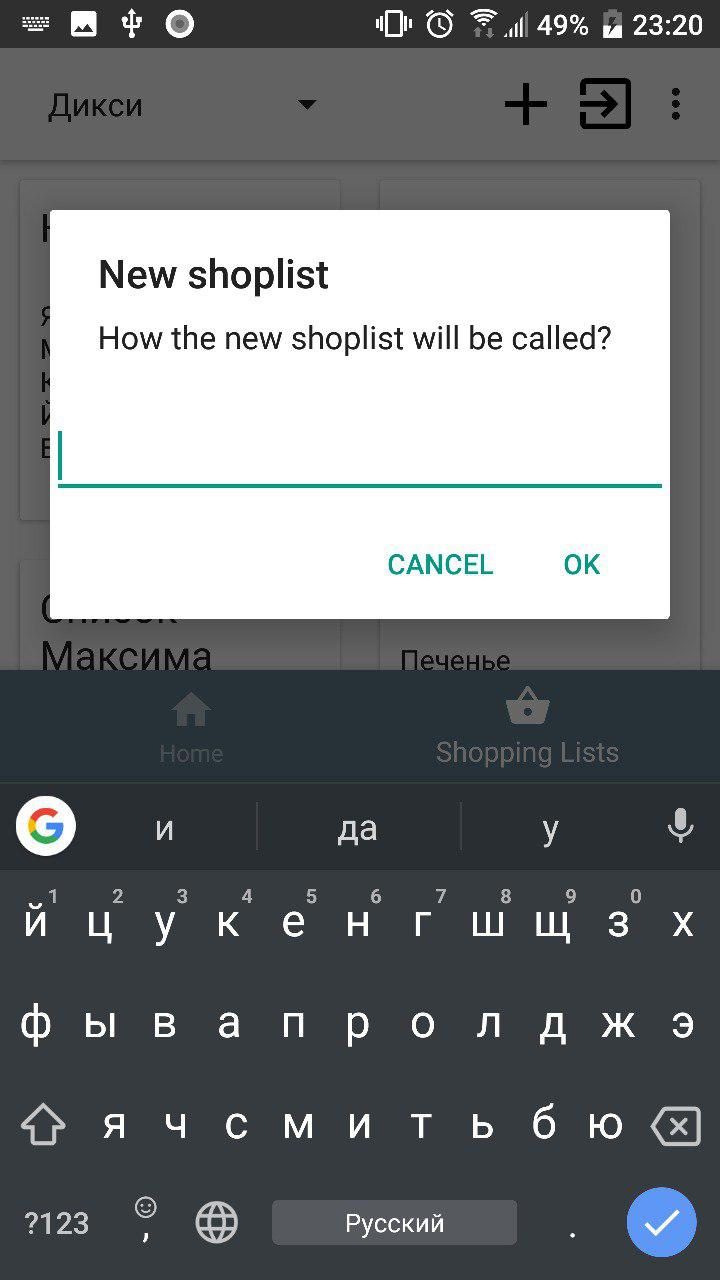
\includegraphics[height=0.38\textheight]{./screenshots/3/new_shoplist.jpg}
    \caption{\small{создание нового списка покупок}}
    \endminipage\hfill
    \minipage{0.3\textwidth}
    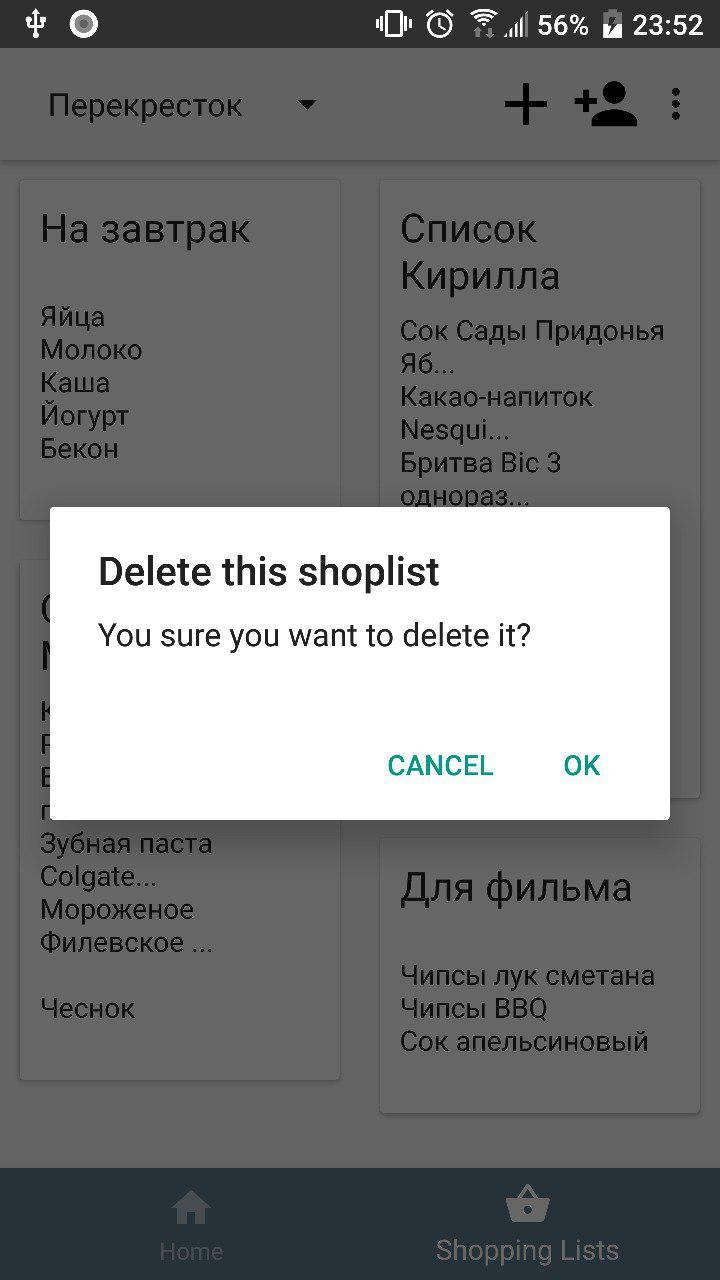
\includegraphics[height=0.38\textheight]{./screenshots/3/delete_shoplist.jpg}
    \caption{\small{удаление списка покупок}}
    \label{delete_sl}
    \endminipage{}
\end{figure}

Добавление товара в список покупок должна вызываться нажатием кнопки '+', а
удалениe товара из списка покупок путём нажатия кнопки '-'.

Добавление в список
покупок пользовательских товаров, которых нет в магазине вызывается нажатием
'+' из списка покупок, а просмотр подобранных программой товаров согласно
запросу пользователя должен вызываться нажатием на пользовательский товар.
Рис~\ref{custom}

При долгом зажатии подобранных товаров должно происходить добавление
подобранных товаров в список покупок.

При переходе на фрагмент 2 (Списки покупок), на экране устройства должно
показываться предварительное отображение элементов каждого списка покупок до их
открытия.

\begin{figure}[h!]
    \centering
    \minipage{0.3\textwidth}
    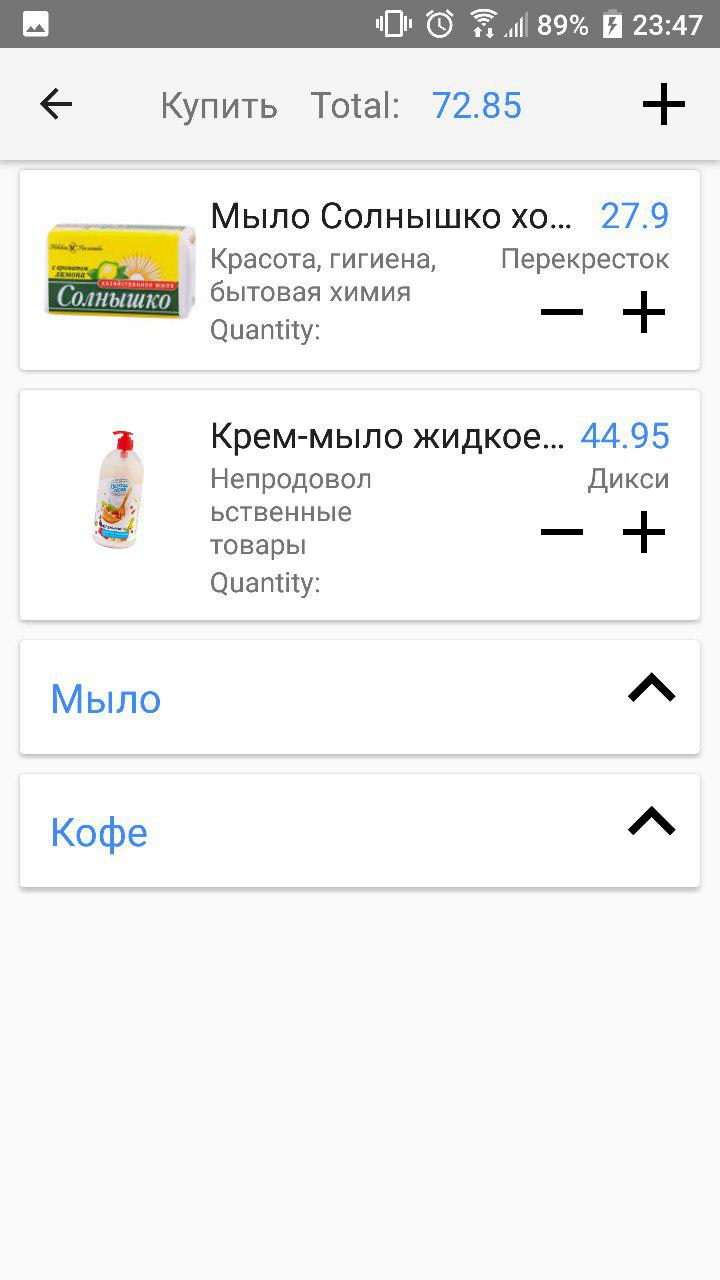
\includegraphics[height=0.38\textheight]{./screenshots/3/shoplist.jpg}
    \caption{\small{просмотр конкретного списка покупок}}
    \endminipage\hfill
    \minipage{0.3\textwidth}
    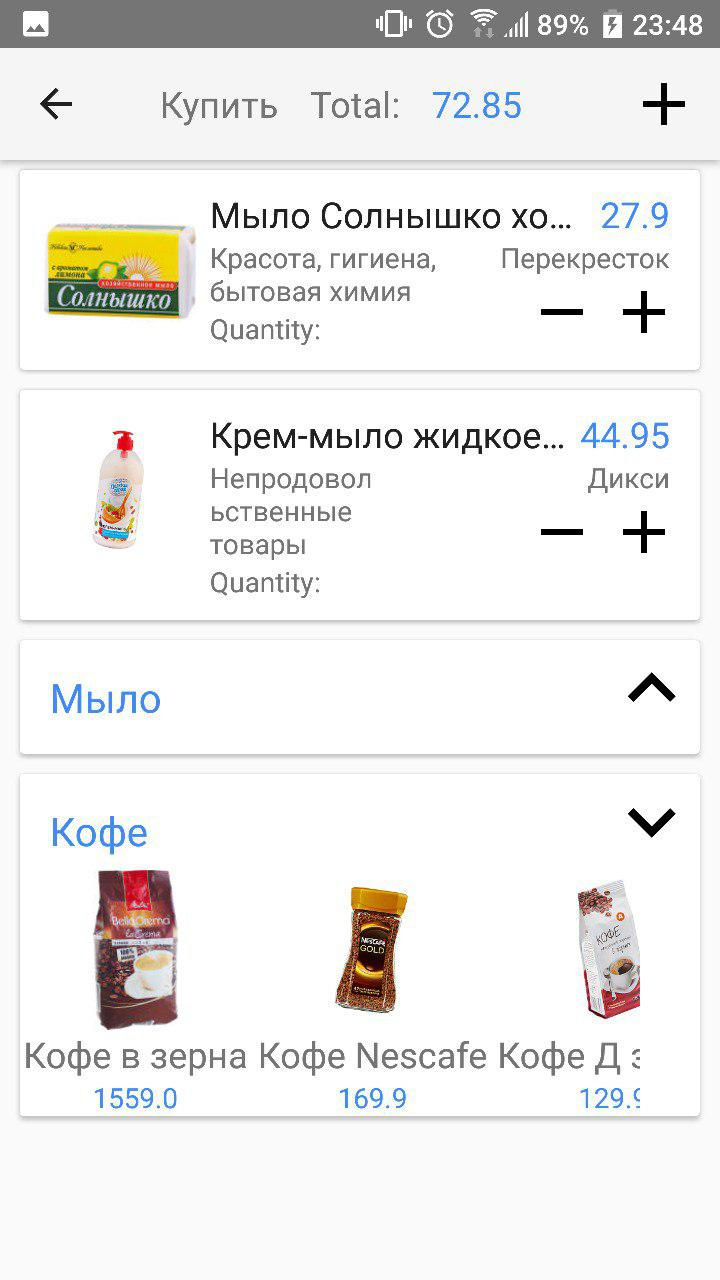
\includegraphics[height=0.38\textheight]{./screenshots/3/shoplist_custom_fold.jpg}
    \caption{\small{просмотр подобранных программой товаров в соответствии с запросом пользователя}}
    \label{custom}
    \endminipage\hfill
    \minipage{0.3\textwidth}
    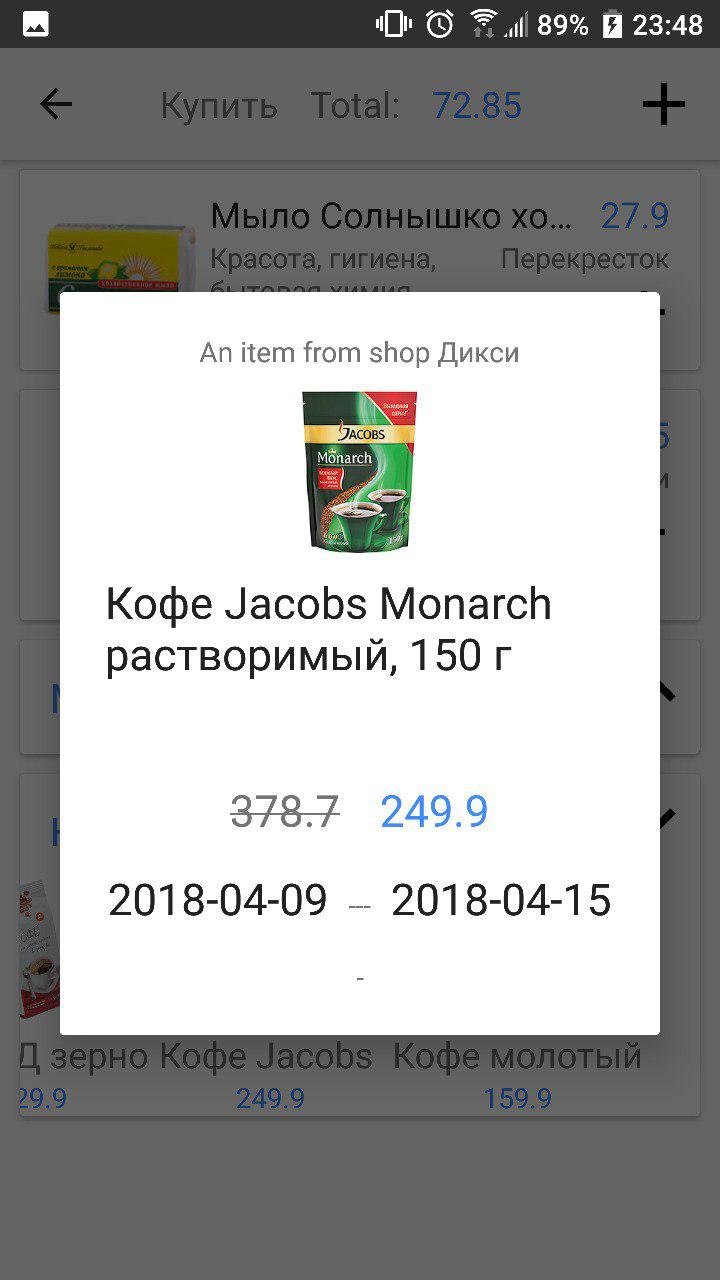
\includegraphics[height=0.38\textheight]{./screenshots/3/full_item_preview.jpg}
    \caption{\small{просмотр всей информации о товаре}}
    \endminipage{}
\end{figure}

На экране с активностью RegisterActivity (Рис.~\ref{register}) должна быть возможность регистрации
через мобильное приложение, а на экране LoginActivity (Рис.~\ref{register}) --- вход в аккаунт через
мобильное приложение, возможность смены аккаунта должна осуществляться путём 1) выхода из аккаунта 2) входа в другой аккаунт.

\begin{figure}[h!]
    \centering
    \minipage{0.45\textwidth}
    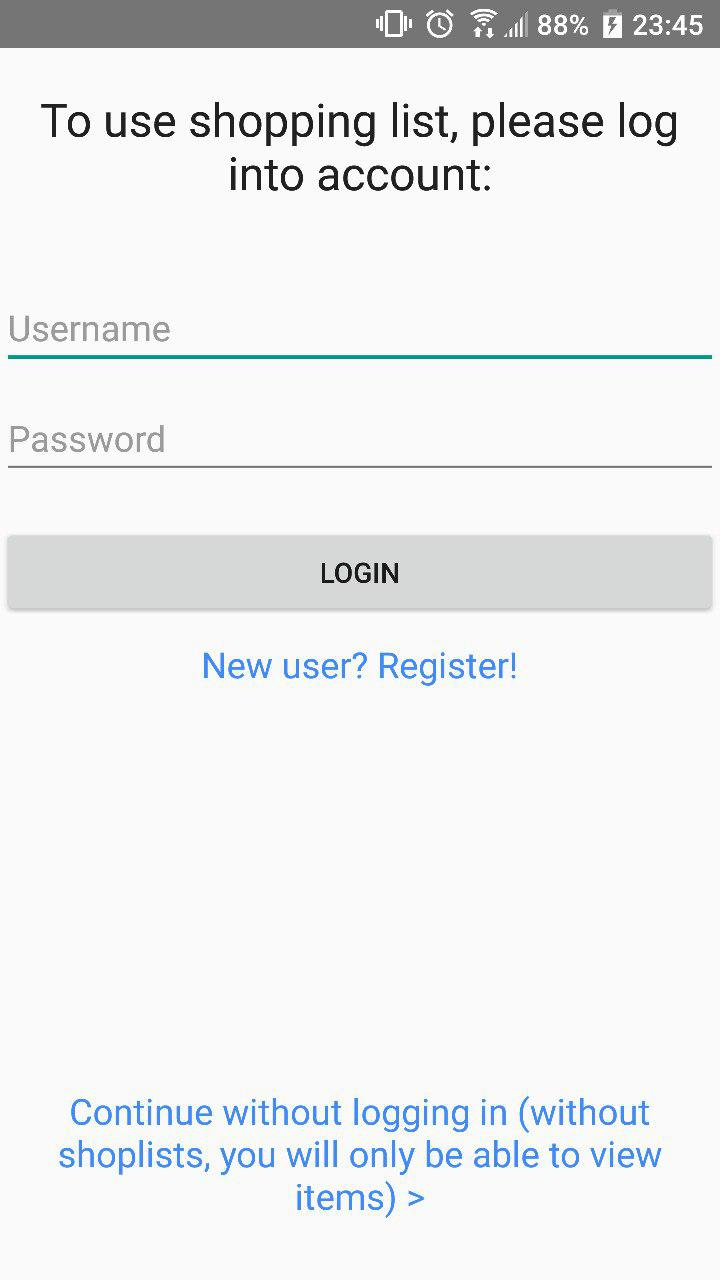
\includegraphics[height=0.42\textheight]{./screenshots/3/login.jpg}
    \caption{\small{вход в аккаунт}}
    \label{login}
    \endminipage\hfill
    \minipage{0.45\textwidth}
    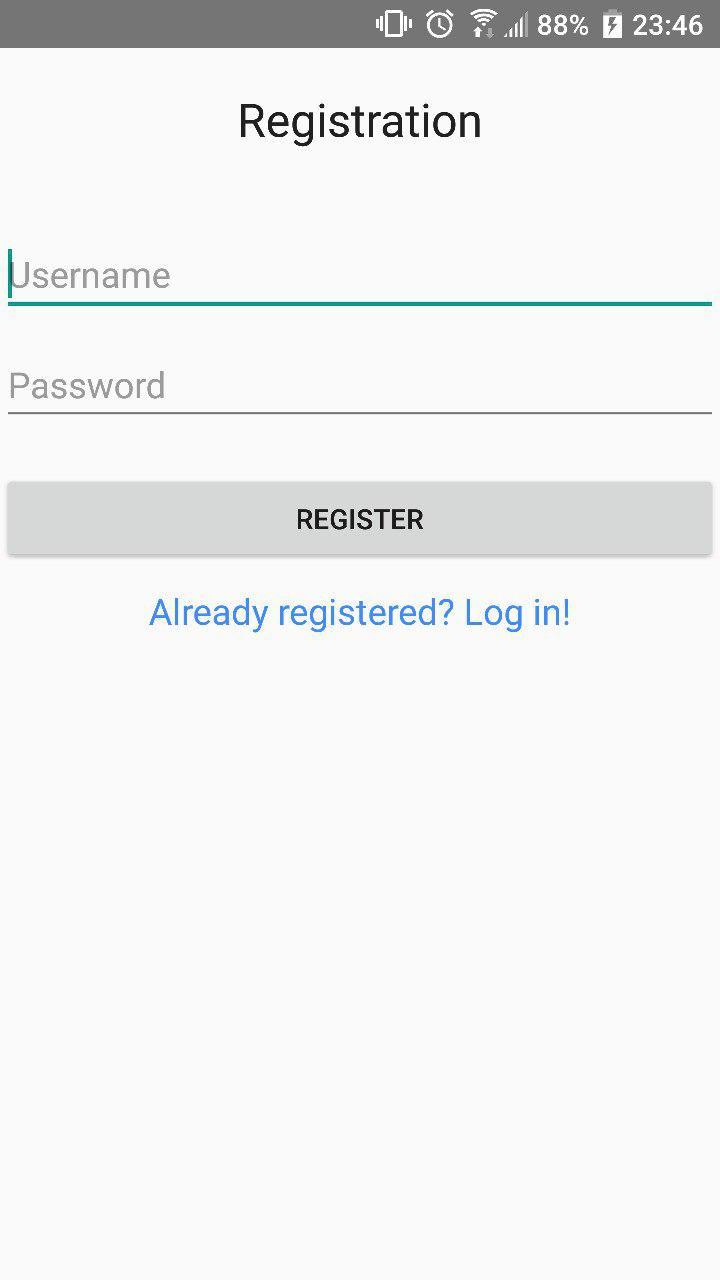
\includegraphics[height=0.42\textheight]{./screenshots/3/register.jpg}
    \caption{\small{регистрация аккаунта}}
    \label{register}
    \endminipage{}
\end{figure}


При долгом нажатии на элементы
управления button (кнопка) должны появляться всплывающие подсказки. (Рис.~\ref{hint})

Должен быть реализован обучающий фрагмент в разделе help (), содержащий руководство
пользователя по управлению программой. (Рис.~\ref{help})
Должно быть отображение индикатора процесса загрузки данных с сервера,
При отсутствии интернет-соединения должно происходить перенаправление в настройки сети для
последующего включения интернета .

\begin{figure}[h!]
    \centering
    \minipage{0.3\textwidth}
    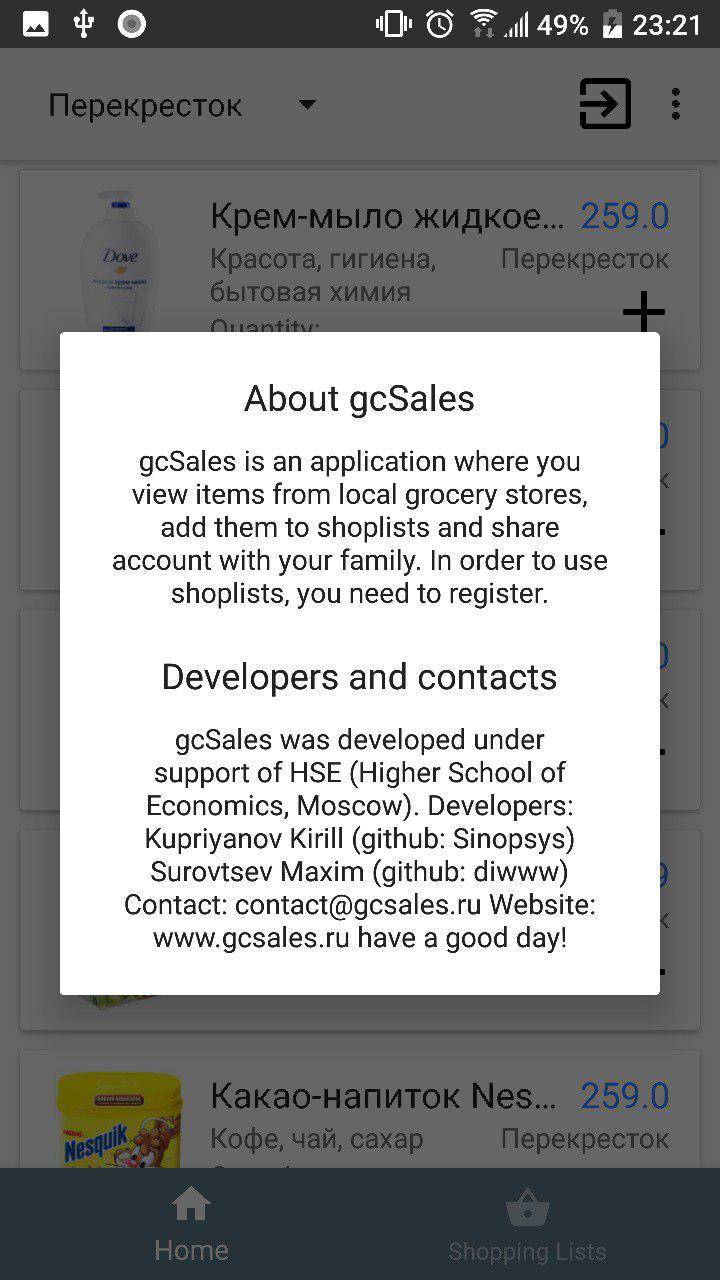
\includegraphics[height=0.38\textheight]{./screenshots/3/about.jpg}
    \caption{\small{просмотр раздела ``о приложении''}}
    \endminipage\hfill
    \minipage{0.3\textwidth}
    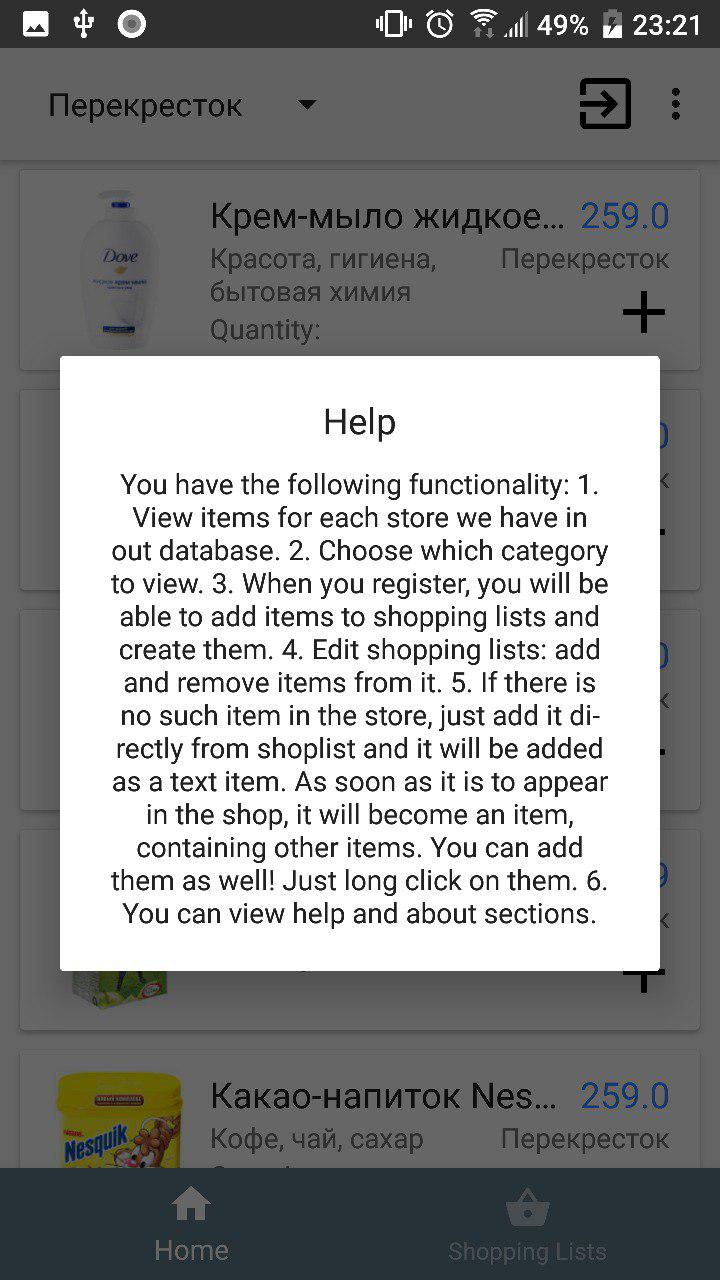
\includegraphics[height=0.38\textheight]{./screenshots/3/help.jpg}
    \caption{\small{просмотр подсказки пользования приложением}}
    \label{help}
    \endminipage\hfill
    \minipage{0.3\textwidth}
    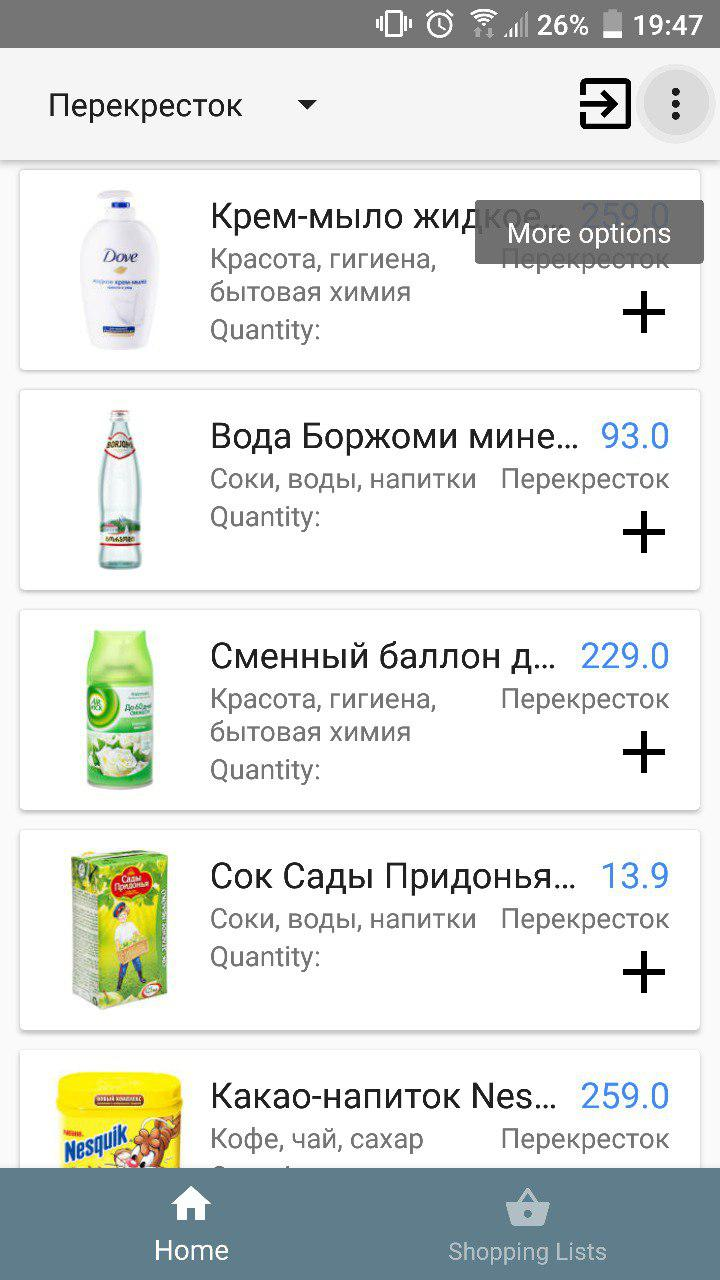
\includegraphics[height=0.38\textheight]{./screenshots/3/hint.jpg}
    \caption{\small{просмотр всплывающего описания элементов button (кнопок)}}
    \label{hint}
    \endminipage{}
\end{figure}

\newpage
\subsubsection{Crawler}
Все необходимые для реализации программы модули должны быть реализованы (Рис.~\ref{tree})

\begin{figure}[h!]
    \centering
    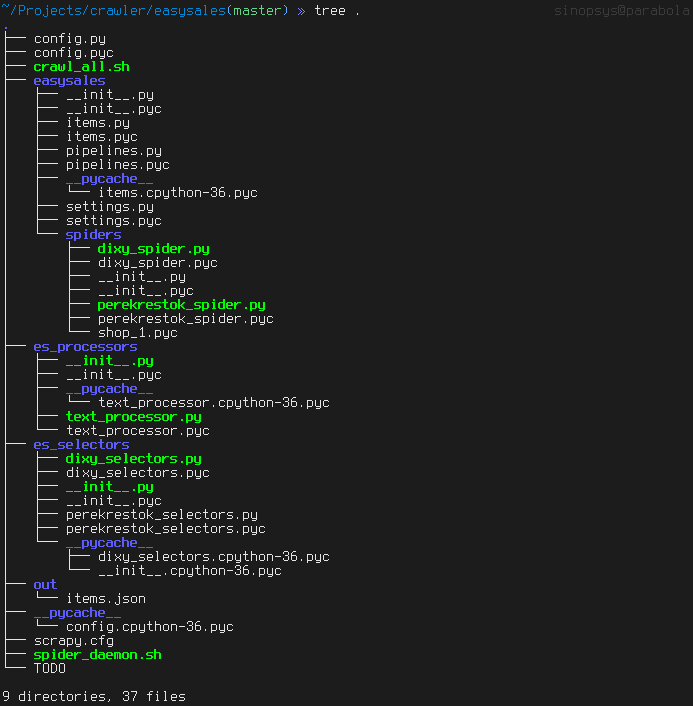
\includegraphics[width=0.56\textwidth]{./screenshots/3/tree.png}
    \caption{\small{структура проекта crawler'a}}
    \label{tree}
\end{figure}

\newpage
Работа crawler'a на Рис.~\ref{crawl_dixy}. При запуске всё работает должно
работать по описанному в настоящей Пояснительной Записке алгоритму, запросы
должны отправляться на сервер.

\begin{figure}[h!]
    \centering
    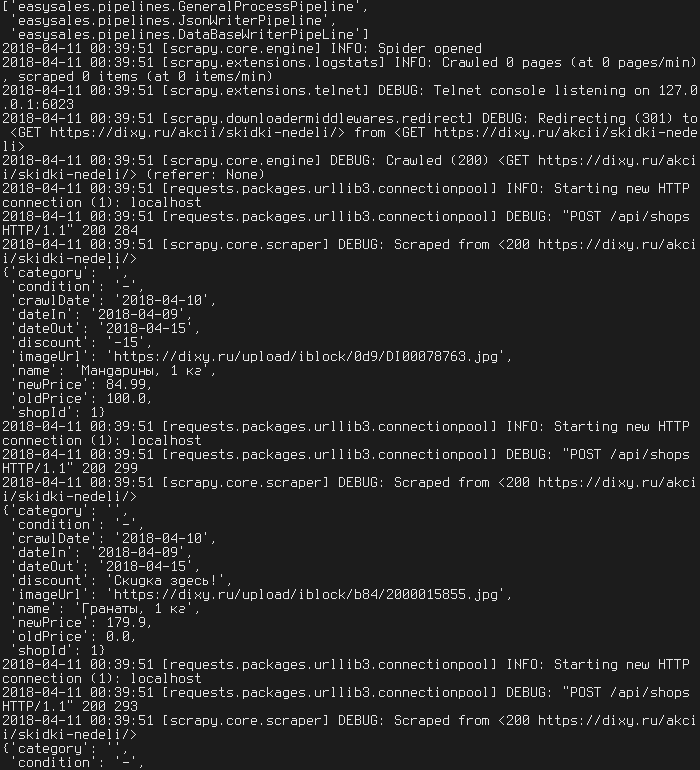
\includegraphics[width=0.9\textwidth]{./screenshots/3/crawl_dixy.png}
    \caption{\small{начало запуска crawler'a}}
    \label{crawl_dixy}
\end{figure}


\newpage
\subsection{Проверка требований к временным характеристикам}
\subsubsection{Андроид приложение}
Будут приводится log-сообщения (см. терминологию) из используемого средства разработки.

Время запуска приложения не должно превышать двух секунд (Рис.~\ref{launch})

\begin{figure}[h!]
    \centering
    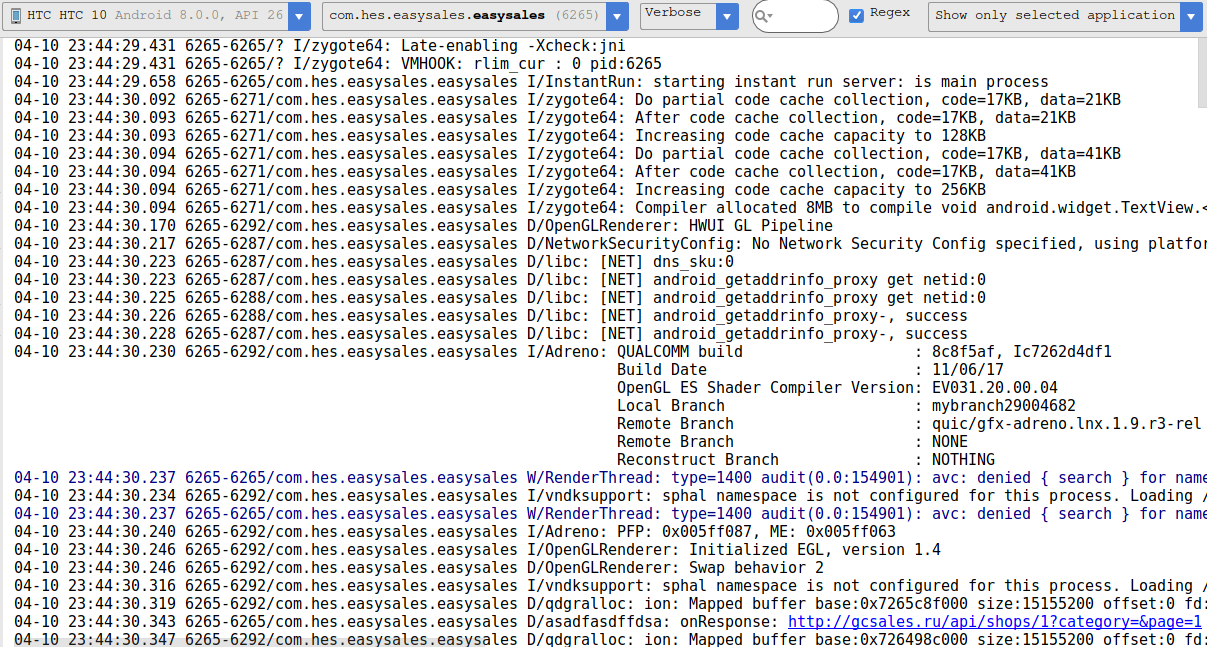
\includegraphics[width=0.9\textwidth]{./screenshots/3/lauch_log.png}
    \caption{\small{log. Запуск приложения}}
    \label{launch}
\end{figure}


Время загрузки одной страницы акций не должно превышать двух секунд (Рис.~\ref{loading})

\begin{figure}[h!]
    \centering
    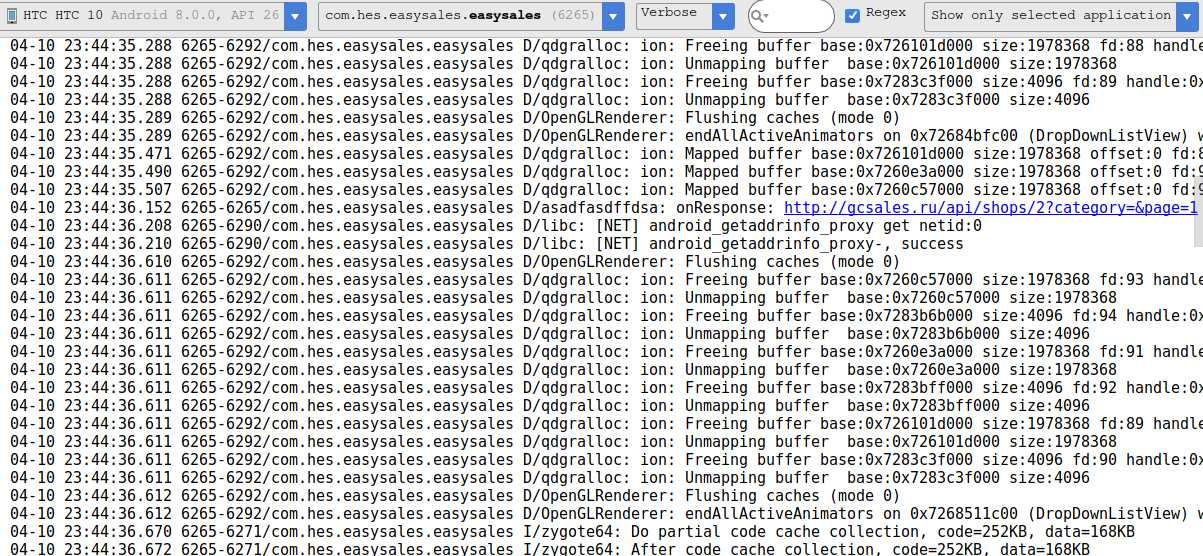
\includegraphics[width=0.9\textwidth]{./screenshots/3/load_log.png}
    \caption{\small{log. Загрузка акций}}
    \label{loading}
\end{figure}
Все временные требования должны быть соблюдены.
\subsubsection{Crawler}
Временные требования к работе crawler'a не предъявлялись.
